\section{The Slice Language and Type System}\label{sec:language}

The syntax of the \Slice{} language is shown in Figure~\ref{fig:grammar}.

\begin{figure}[h]
\begin{align*}
e ::= &\; x                               & \text{variable} \\
    | &\; c                               & \text{float constant} \\
    | &\; \text{true} \mid \text{false}   & \text{boolean constant} \\
    | &\; \finconst{k}{n}                 & \text{finite type constant (k of type fin(n))} \\
    | &\; ()                              & \text{unit} \\
    | &\; \letkw \; x = e_1\; \inkw \; e_2  & \text{let binding} \\
    | &\; \text{cdistr}                   & \text{continuous distribution} \\
    | &\; \discrete(p_0, \ldots, p_{n})      & \text{discrete distribution} \\
    | &\; e_1 < e_2                       & \text{less-than (floats)} \\
    | &\; e_1 \leq e_2                    & \text{less-or-equal (integers)} \\
    | &\; e_1 \finlt{n} e_2              & \text{less-than (finite type n)} \\
    | &\; e_1 \finleq{n} e_2             & \text{less-or-equal (finite type n)} \\
    | &\; e_1 \logand e_2                 & \text{logical and} \\
    | &\; e_1 \logor e_2                  & \text{logical or} \\
    | &\; \text{not}\; e                  & \text{logical not} \\
    | &\; \ifkw \; e_1\; \thenkw \; e_2\; \elsekw \; e_3 & \text{conditional} \\
    | &\; (e_1, e_2)                      & \text{pair construction} \\
    | &\; \fstkw \; e                     & \text{first projection} \\
    | &\; \sndkw \; e                     & \text{second projection} \\
    | &\; \funkw \; x \; \rightarrow \; e & \text{function abstraction} \\
    | &\; e_1 \; e_2                      & \text{function application} \\
    | &\; \text{fix}\; f\; x := e         & \text{fixed-point recursion} \\
    | &\; \text{observe}\; e              & \text{observation/conditioning} \\
    | &\; e_1; e_2                        & \text{sequencing} \\
    | &\; \text{nil}                      & \text{empty list} \\
    | &\; e_1 :: e_2                      & \text{list cons} \\
    | &\; \text{match}\; e\; \text{with}\; \text{nil} \rightarrow e_1 \mid h :: t \rightarrow e_2\; \text{end} & \text{list match} \\
    | &\; \text{ref}\; e                  & \text{reference creation} \\
    | &\; !e                              & \text{dereference} \\
    | &\; e_1 := e_2                      & \text{assignment} \\
    \\[1ex] % Add some space before cdistr definition
\text{cdistr} ::= &\; \uniform(e_1, e_2)      & \text{uniform distribution} \\
           | &\; \gaussian(e_1, e_2)   & \text{gaussian distribution} \\
           | &\; \exponential(e)       & \text{exponential distribution} \\
           | &\; \betafn(e_1, e_2)     & \text{beta distribution} \\
           | &\; \ldots                & \text{(and 13+ more distributions)}
\end{align*}
\caption{Syntax of the \Slice{} language.}
\label{fig:grammar}
\end{figure}

\noindent where $x$ ranges over variable names, $c$ ranges over floating point constants, $i$ ranges over integer constants, $k$ and $n$ are non-negative integers with $0 \leq k < n$, $h$ and $t$ are variables in list patterns, and $p_0, \ldots, p_n$ are probabilities that should sum to 1.

The uniform distribution $\uniform(e_1, e_2)$ represents a continuous random value uniformly distributed in the range $[e_1, e_2)$. Other continuous distributions are defined according to their standard statistical definitions. The implementation supports over 17 distributions including Gaussian, exponential, beta, gamma, Laplace, Cauchy, and others. The discrete distribution $\discrete(p_0, \ldots, p_{n})$ represents a random value that returns integer $i \in \{0, \ldots, n\}$ with probability $p_i$.

Beyond basic functional constructs (pairs, projections, lambda abstractions, and function application), the language includes:
\begin{itemize}
\item \textbf{Finite types}: Values of the form $\finconst{k}{n}$ represent finite type constants, where $k$ is a value in the finite type with $n$ elements.
\item \textbf{Boolean operations}: Logical operators $\logand$, $\logor$, and $\text{not}$ for boolean expressions.
\item \textbf{Fixed-point recursion}: The $\text{fix}$ construct enables recursive function definitions.
\item \textbf{Observations}: The $\text{observe}$ construct conditions the program on a boolean expression being true.
\item \textbf{Lists}: Constructed with $\text{nil}$ and $::$, and deconstructed with pattern matching.
\item \textbf{Mutable references}: Created with $\text{ref}$, dereferenced with $!$, and updated with $:=$.
\item \textbf{Sequencing}: The semicolon operator sequences expressions with side effects.
\end{itemize}

When we discretize continuous programs, we convert expressions involving continuous distributions into expressions with discrete distributions, and convert less-than comparisons into less-than-or-equal comparisons on the corresponding discrete intervals.

\subsection{Type System}\label{sec:type-system}

We introduce a type system that analyzes both the comparison points and concrete values of floating point expressions. We have the following types:
\begin{itemize}
    \item \bool: the expression is a boolean value (true or false)
    \item \intty: the expression is an integer value  
    \item $\fin{n}$: the expression is a finite type value in $\{0, 1, \ldots, n-1\}$
    \item \float$\langle B; V \rangle$: the expression is a floating point value with comparison bounds $B$ and value set $V$
    \item $\tau_1 * \tau_2$: the expression is a pair with elements of type $\tau_1$ and $\tau_2$
    \item $\tau_1 \rightarrow \tau_2$: the expression is a function that takes an argument of type $\tau_1$ and returns a result of type $\tau_2$
    \item $\text{unit}$: the unit type with single value $()$
    \item $\text{list}(\tau)$: list of elements of type $\tau$
    \item $\text{ref}(\tau)$: mutable reference containing a value of type $\tau$
\end{itemize}

The float type \float$\langle B; V \rangle$ uses a two-bag approach:
\begin{itemize}
    \item $B$ is the \emph{bound bag}, containing comparison bounds of the form $< c$ or $\leq c$
    \item $V$ is the \emph{value bag}, containing concrete float values that the expression can evaluate to
\end{itemize}

Both $B$ and $V$ can be either a finite set or $\top$ (representing an unknown/unbounded set). This forms a product lattice structure that we describe in detail below.

\subsubsection{Lattice Structure}

Each bag forms a join-semilattice with the following structure:
\begin{itemize}
    \item Elements: $\{\text{Finite}(S) \mid S \text{ is a finite set}\} \cup \{\top\}$
    \item Ordering: $\text{Finite}(S_1) \sqsubseteq \text{Finite}(S_2)$ if $S_1 \subseteq S_2$, and $\text{Finite}(S) \sqsubseteq \top$ for any $S$
    \item Join: $\text{Finite}(S_1) \sqcup \text{Finite}(S_2) = \text{Finite}(S_1 \cup S_2)$, and $x \sqcup \top = \top$ for any $x$
    \item Bottom: $\text{Finite}(\emptyset)$
    \item Top: $\top$
\end{itemize}

The float type forms a product lattice:
\begin{align}
\text{FloatLattice} &= \text{BoundLattice} \times \text{ValueLattice} \\
(B_1, V_1) \sqsubseteq (B_2, V_2) &\iff B_1 \sqsubseteq B_2 \land V_1 \sqsubseteq V_2 \\
(B_1, V_1) \sqcup (B_2, V_2) &= (B_1 \sqcup B_2, V_1 \sqcup V_2)
\end{align}

This product lattice is also a join-semilattice with:
\begin{itemize}
    \item Bottom element: $(\text{Finite}(\emptyset), \text{Finite}(\emptyset))$
    \item Top element: $(\top, \top)$
\end{itemize}

The lattice structure enables type inference to systematically collect and propagate information about both how values are used (bounds) and what values they can take (values).

\begin{figure}[!t]
\centering
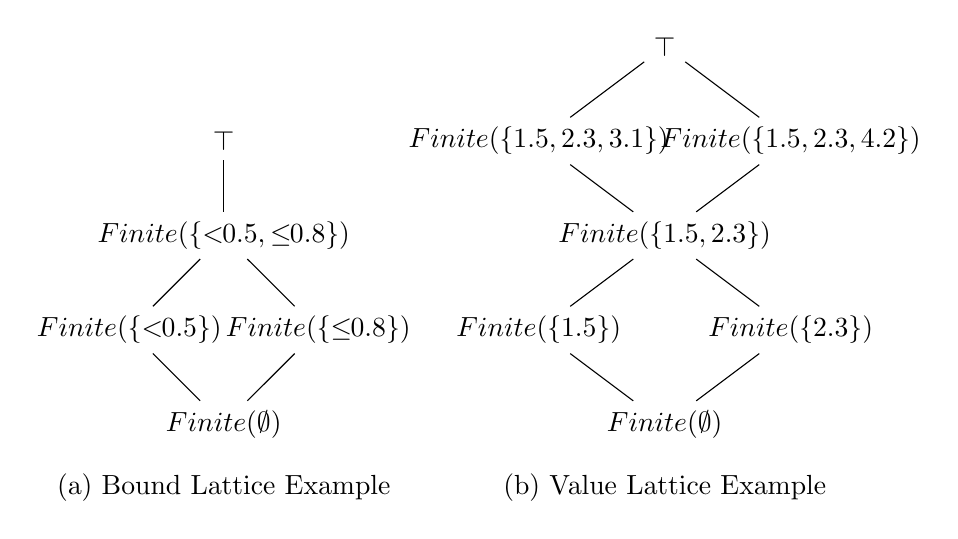
\begin{tikzpicture}[scale=0.8]
  % Individual lattice (left)
  \node (bot1) at (0,0) {$\text{Finite}(\emptyset)$};
  \node (s1) at (-1.5,1.5) {$\text{Finite}(\{<\!\!0.5\})$};
  \node (s2) at (1.5,1.5) {$\text{Finite}(\{\leq\!\!0.8\})$};
  \node (s12) at (0,3) {$\text{Finite}(\{<\!\!0.5, \leq\!\!0.8\})$};
  \node (top1) at (0,4.5) {$\top$};
  
  \draw (bot1) -- (s1);
  \draw (bot1) -- (s2);
  \draw (s1) -- (s12);
  \draw (s2) -- (s12);
  \draw (s12) -- (top1);
  
  \node at (0,-1) {(a) Bound Lattice Example};
  
  % Product lattice (right)
  \node (bot2) at (7,0) {$\text{Finite}(\emptyset)$};
  \node (s3) at (5,1.5) {$\text{Finite}(\{1.5\})$};
  \node (s4) at (9,1.5) {$\text{Finite}(\{2.3\})$};
  \node (s34) at (7,3) {$\text{Finite}(\{1.5, 2.3\})$};
  \node (s5) at (5,4.5) {$\text{Finite}(\{1.5, 2.3, 3.1\})$};
  \node (s6) at (9,4.5) {$\text{Finite}(\{1.5, 2.3, 4.2\})$};
  \node (top2) at (7,6) {$\top$};
  
  \draw (bot2) -- (s3);
  \draw (bot2) -- (s4);
  \draw (s3) -- (s34);
  \draw (s4) -- (s34);
  \draw (s34) -- (s5);
  \draw (s34) -- (s6);
  \draw (s5) -- (top2);
  \draw (s6) -- (top2);
  \node at (7,-1) {(b) Value Lattice Example};
\end{tikzpicture}
\caption{Lattice structure for float types. (a) shows an example bound lattice with comparison bounds. (b) the lattice over real values.}
\label{fig:lattice}
\end{figure}

The typing rules are as follows:

\begin{mathpar}
    \inferrule[\textsc{Var}]
    {\ }
    {\Gamma, x: \tau \vdash x : \tau}

    \inferrule[\textsc{Let}]
    {\Gamma \vdash e_1 : \tau_1 \\
     \Gamma, x: \tau_1 \vdash e_2 : \tau_2}
    {\Gamma \vdash \letkw \; x = e_1 \; \inkw \; e_2 : \tau_2}

    \inferrule[\textsc{If}]
    {\Gamma \vdash e_1 : \bool \\
     \Gamma \vdash e_2 : \tau \\
     \Gamma \vdash e_3 : \tau}
    {\Gamma \vdash \ifkw \; e_1 \; \thenkw \; e_2 \; \elsekw \; e_3 : \tau}

    \inferrule[\textsc{Float}]
    {\ c \in V }
    {\Gamma \vdash c : \float\langle B; V \rangle}

    \inferrule[\textsc{ContDist}]
    {\ }
    {\Gamma \vdash cdistr : \float\langle B; \top \rangle}

    \inferrule[\textsc{Discrete}]
    {\ }
    {\Gamma \vdash \discrete(p_0, \ldots, p_n) : \fin{n}}

    \inferrule[\textsc{Less}]
    {\Gamma \vdash e : \float\langle B; V \rangle}
    {\Gamma \vdash e < c : \bool}
    \quad \text{where } B \text{ is constrained to include } {<c}

    \inferrule[\textsc{LessEq}]
    {\Gamma \vdash e : \intty}
    {\Gamma \vdash e \leq i : \bool}

    \inferrule[\textsc{Pair}]
    {\Gamma \vdash e_1 : \tau_1 \\
     \Gamma \vdash e_2 : \tau_2}
    {\Gamma \vdash (e_1, e_2) : \tau_1 * \tau_2}

    \inferrule[\textsc{Fst}]
    {\Gamma \vdash e : \tau_1 * \tau_2}
    {\Gamma \vdash \fstkw \; e : \tau_1}

    \inferrule[\textsc{Snd}]
    {\Gamma \vdash e : \tau_1 * \tau_2}
    {\Gamma \vdash \sndkw \; e : \tau_2}

    \inferrule[\textsc{Fun}]
    {\Gamma, x: \tau_1 \vdash e : \tau_2}
    {\Gamma \vdash \funkw \; x \; \rightarrow \; e : \tau_1 \rightarrow \tau_2}

    \inferrule[\textsc{App}]
    {\Gamma \vdash e_1 : \tau_1 \rightarrow \tau_2 \\
     \Gamma \vdash e_2 : \tau_1}
    {\Gamma \vdash e_1 \; e_2 : \tau_2}

    \inferrule[\textsc{True}]
    {\ }
    {\Gamma \vdash \text{true} : \bool}

    \inferrule[\textsc{False}]
    {\ }
    {\Gamma \vdash \text{false} : \bool}

    \inferrule[\textsc{And}]
    {\Gamma \vdash e_1 : \bool \\
     \Gamma \vdash e_2 : \bool}
    {\Gamma \vdash e_1 \logand e_2 : \bool}

    \inferrule[\textsc{Or}]
    {\Gamma \vdash e_1 : \bool \\
     \Gamma \vdash e_2 : \bool}
    {\Gamma \vdash e_1 \logor e_2 : \bool}

    \inferrule[\textsc{Not}]
    {\Gamma \vdash e : \bool}
    {\Gamma \vdash \text{not}\; e : \bool}

    \inferrule[\textsc{Unit}]
    {\ }
    {\Gamma \vdash () : \text{unit}}

    \inferrule[\textsc{FinConst}]
    {0 \leq k < n}
    {\Gamma \vdash \finconst{k}{n} : \fin{n}}

    \inferrule[\textsc{FinLess}]
    {\Gamma \vdash e_1 : \fin{n} \\
     \Gamma \vdash e_2 : \fin{n}}
    {\Gamma \vdash e_1 \finlt{n} e_2 : \bool}

    \inferrule[\textsc{FinLessEq}]
    {\Gamma \vdash e_1 : \fin{n} \\
     \Gamma \vdash e_2 : \fin{n}}
    {\Gamma \vdash e_1 \finleq{n} e_2 : \bool}

    \inferrule[\textsc{Observe}]
    {\Gamma \vdash e : \bool}
    {\Gamma \vdash \text{observe}\; e : \text{unit}}

    \inferrule[\textsc{Seq}]
    {\Gamma \vdash e_1 : \tau_1 \\
     \Gamma \vdash e_2 : \tau_2}
    {\Gamma \vdash e_1; e_2 : \tau_2}

    \inferrule[\textsc{Fix}]
    {\Gamma, f: \tau_1 \rightarrow \tau_2, x: \tau_1 \vdash e : \tau_2}
    {\Gamma \vdash \text{fix}\; f\; x := e : \tau_1 \rightarrow \tau_2}

    \inferrule[\textsc{Nil}]
    {\ }
    {\Gamma \vdash \text{nil} : \text{list}(\tau)}

    \inferrule[\textsc{Cons}]
    {\Gamma \vdash e_1 : \tau \\
     \Gamma \vdash e_2 : \text{list}(\tau)}
    {\Gamma \vdash e_1 :: e_2 : \text{list}(\tau)}

    \inferrule[\textsc{Match}]
    {\Gamma \vdash e : \text{list}(\tau_1) \\
     \Gamma \vdash e_1 : \tau_2 \\
     \Gamma, h: \tau_1, t: \text{list}(\tau_1) \vdash e_2 : \tau_2}
    {\Gamma \vdash \text{match}\; e\; \text{with}\; \text{nil} \rightarrow e_1 \mid h :: t \rightarrow e_2\; \text{end} : \tau_2}

    \inferrule[\textsc{Ref}]
    {\Gamma \vdash e : \tau}
    {\Gamma \vdash \text{ref}\; e : \text{ref}(\tau)}

    \inferrule[\textsc{Deref}]
    {\Gamma \vdash e : \text{ref}(\tau)}
    {\Gamma \vdash !e : \tau}

    \inferrule[\textsc{Assign}]
    {\Gamma \vdash e_1 : \text{ref}(\tau) \\
     \Gamma \vdash e_2 : \tau}
    {\Gamma \vdash e_1 := e_2 : \text{unit}}
\end{mathpar}

